% !TeX root = mos-he.tex

%%%%%%%%%%%%%%%%%%%%%%%%%%%%%%%%%%%%%%%%%%%%%%%%%%%%%%%%%%%%%

\selectlanguage{hebrew}

\begin{center}
\textbf{\Large בעיות ופתרונות}
\end{center}

\addcontentsline{toc}{section}{\large בעיות ופתרונות}

\begin{prob}{מגרת הגרביים}{S}{The sock drawer}
%\begin{prob}{ מגרת הגרביים\annotate{S} \L{\small (The sock drawer)}}
במגרה נמצאות גרביים אדומות וגרביים שחורות. אם נשלוף שתי גרביים בצורה אקראית
\textbf{(עם החזרה)}
ההסתברות ששתיהן אדומות היא
$\frac{1}{2}$. 

\que{1}
מה המספר הקטן ביותר של גרביים שחורות שיכולות להיות במגרה? עבור מספר זה מה מספר הגרביים האדומות?

\que{2}
מה המספר 
\textbf{הזוגי}
הקטן ביותר של גרביים שחורות שיכולות להיות במגרה? עבור מספר זה מה מספר הגרביים האדומות?

\end{prob}

\solution{1}

\ans{1}
יהי
$r$
מספר הגרביים האדומות במגירה ויהי 
$b$
מספר הגרביים השחורות. 
$r\geq 2$
כי נתון שניתן לשלוף שתי גרביים אדומות, ו-%
$b\geq 1$
אחרת ההסתברות של שליפת שתי גרביים אדומות היה 
$1$.
נכפיל את ההסתברויות של שתי השליפות:
\begin{equation}\label{eq.1-a}
P(\textrm{אדומים שניים})=\frac{r}{r+b} \cdot \frac{(r-1)}{(r-1)+b} = \frac{1}{2}\,.
\end{equation}
נפשט ונקבל משוואה ריבועית עבור המשתנה 
$r$:
\begin{equation}\label{eq.quad-for-r}
r^2-r(2b+1)-(b^2-b)=0\,.
\end{equation}
$r,b$
שנייהם מספרים שלמים חיוביים ולכן הדיסקרימיננט חייב להיות ריבוע של מספר שלם:
\begin{equation}\label{eq.discriminant}
(2b+1)^2+4(b^2-b)=8b^2+1
\end{equation}
הדיסקרימיננט הוא ריבוע כאשר 
$b=1$
(הערך הקטן ביותר). ממשוואה%
~$\ref{eq.quad-for-r}$, $r=3$,
כאשר אנו דוחים את הפתרון 
$r=0$
כי
$r\geq 2$.
סכום מספר הגרביים הוא 
$4$.

בדיקה:
$\frac{3}{4}\cdot\frac{2}{3}=\frac{1}{2}$.

\medskip

\ans{2}
בדקו כל מספר שלם חיובי זוגית של 
$b$
כדי למצוא את המספר הקטן ביותר עבורו הדיסקרימיננט הוא ריבוע:
\begin{displaymath}
\renewcommand{\arraystretch}{1}
\begin{array}{r|r|r}
b&8b^2+1&\sqrt{8b^2+1}\\
\hline
2&33&5.74\\
4&129&11.36\\
\mathbf{6}&\mathbf{289}&\mathbf{17}
\end{array}
\end{displaymath}
עבור
$b=6$ 
הערך של 
$r$
הוא
$15$
שמתקבל על ידי פתרון משוואה%
~$\ref{eq.quad-for-r}$.

בדיקה:
$\frac{15}{21}\cdot\frac{14}{20}=\frac{1}{2}$.

\solution{2}

\ans{1}
האם אי-שוויון זה נכון?
\begin{equation}\label{eq.1-b}
\frac{r}{r+b} \stackrel{?}{>} \frac{r-1}{(r-1)+b}\,.
\end{equation}
$r\geq 2, b\geq 1$
ולכן שני המכנים חיוביים וניתן להכפיל את שני הצדדים:
\begin{eqnarray*}
r(r-1+b)&\stackrel{?}{>}&(r-1)(r+b)\\
r^2-r+rb&\stackrel{?}{>}&r^2-r+rb-b\\
b&\stackrel{?}{>}&0\,.
\end{eqnarray*}
$b>1$
כך שמשווה%
~$\ref{eq.1-b}$
נכונה.

לפי משוואות%
~$\ref{eq.1-a}, \ref{eq.1-b}$:
\begin{equation}\label{eq.1-c}
\left(\frac{r}{r+b}\right)^2 = \frac{r}{r+b} \cdot\frac{r}{r+b} > \frac{r}{r+b} \cdot \frac{r-1}{(r-1)+b} = \frac{1}{2}\,,
\end{equation}
ובאופן דומה:
\begin{equation}\label{eq.1-d}
\left(\frac{r-1}{(r-1)+b}\right)^2  = \frac{r-1}{(r-1)+b}\cdot \frac{r-1}{(r-1)+b}<  \frac{r}{r+b} \cdot \frac{r-1}{(r-1)+b} = \frac{1}{2}\,.
\end{equation}
המכנה
$r+b$
שונה מאפס ולכן ניתן לחשב שורש ריבועי ולפשט את משוואה%
~$\ref{eq.1-c}$:
\begin{eqnarray*}
\frac{r}{r+b}  &>& \sqrt{\frac{1}{2}}\\
r&>&\frac{b}{\sqrt{2}-1}\\
r&>&\frac{b}{\sqrt{2}-1}\cdot\frac{\sqrt{2}+1}{\sqrt{2}+1}\\
r&>&b(\sqrt{2}+1)\,.
\end{eqnarray*}
באופן דומה עבור משוואה%
~$\ref{eq.1-d}$:
\begin{eqnarray*}
\frac{r-1}{(r-1)+b}&<&\sqrt{\frac{1}{2}}\\
r-1 &<& \frac{b}{\sqrt{2}-1}\\
r-1&<&b(\sqrt{2}+1)\,.
\end{eqnarray*}
משתי המשוואות נקבל:
\begin{equation}\label{eq.inequalities}
r-1<(\sqrt{2}+1)b<r\,.
\end{equation}
עבור 
$b=1$
מתקבל
$2.141 < r< 3.141$
ו-%
$b=1,r=3$
הוא פתרון.

\ans{2} 
נבדוק מספרים זוגיים עבור
$b$:
\begin{displaymath}	
\renewcommand{\arraystretch}{1}
\begin{array}{r|ccc|c|c}
b& (\sqrt{2}+1)b&<r<& (\sqrt{2}+1)b+1&r&P(\textrm{שתי אדומות})\\
\hline
2&4.8&<r<&5.8&5&0.4762\\
4&9.7&<r<&10.7&10&0.4945\\
6&14.5&<r<&15.5&
15&0.5000
\end{array}
\end{displaymath}
\L{Mosteller}
מעיר שקיים קשר בין בעיה זו לתורת המספרים ומביא פתרון נוסף:
$b=35,r=85$.


\medskip
\textbf{Simulation}
\selectlanguage{english}
\begin{verbatim}
Expectation of both red  = 0.5000
Average of both red for (red =  3, black =  1) = 0.5053
Average of both red for (red = 15, black =  6) = 0.5013
Average of both red for (red = 85, black = 35) = 0.4961
\end{verbatim}
\selectlanguage{hebrew}

\textbf{הערה}

בשני הפתרונות אנחנו לא מוכיחים תנאי
\emph{מספיק}
עבור הערכים של 
$r,b$.
בפתרון~
$1$
פיתחנו תנאי הכרחי---לפי משוואה%
~$\ref{eq.discriminant}$
הדיסקרימיננט חייב להיות מספר שלם---ומחפשים ערכים של 
$b$
שעומדים בדרישה זו. בפתרון~$2$ התנאי ההכרחי הוא ש-%
$r,b$
מספקים את האי-שוויונות במשוואה%
~$\ref{eq.inequalities}$
ואז חיפשנו ערכים שעומדים בדרישה זו. כתבתי תכנית קצרה לחפש פתרונות בטווח 
$[1,50]$.
התוצאות  עבור ערכים מסביב ל-%
$35$
הן:
\selectlanguage{english}
\begin{verbatim}
32 78  90.52 0.500917
33 80  93.34 0.499368
34 83  96.17 0.501474
35 85  99.00 0.500000
36 87 101.83 0.498601
37 90 104.66 0.500562
\end{verbatim}
\selectlanguage{hebrew}
כאשר הטורים הם (משמאל לימין) מספר הגרביים השחורות, מספר הגרביים האדומות, השורש של הדיסקרימיננט (משוואה%
~$\ref{eq.discriminant}$),
ההסתברות לשלוף שתי גרביים אדומות.

בעזרת תכנית מחשב מצאתי את הפתרונות הבאים עבור מספר גרביים שחורות פחות ממיליון:
\[
\begin{array}{r@{\hspace{2em}}r}
\textrm{שחורות} & \textrm{אדומות}\\\hline
1 & 3 \\
6 & 15\\
35 &  85\\
204 &  493\\
1189 &  2871\\
6930 & 16731\\
40391 &  97513\\
235416 & 568345
\end{array}
\]


%%%%%%%%%%%%%%%%%%%%%%%%%%%%%%%%%%%%%%%%%%%%%%%%%%%%%%%%%%%%%

\begin{prob}{נצחונות עוקבים}{S}{Successive wins}
אתם משחקים סדרה של שלושה משחקים נגד אני יריבים ואתם מנצחים בסדרה אם אתם מנצחים שני משחקים לפחות מתוך השלושה. ההסתברות שאתם מנצחים במשחק נגד שחקן 
$P_1$
היא
$p_1$
וההסתברות שאתם מנצחים במשחק נגד שחקן 
$P_2$
היא
$p_2$.
נתון ש-%
$p_1>p2$.
באיזה המתסריטים שלהן יש לכם סיכוי גדול יותר לנצח בסדרה?
\begin{itemize}
\item 
אתם משחקים נגד 
$P_1,P_2,P_1$
בסדר זה.
\item
אתם משחקים נגד
$P_2,P_1,P_2$
בסדר זה.
\end{itemize}
\end{prob}

\solution{1}

אתם מנצחים אם: (א) אתם מנצחים בשני השחקים הראשונים ומפסידים בשלישי, (ב) אתם מפסידים את המשחק הראשון ומנצחים משחק השני ובמשחק השלישי. (ג) אתם מנצחים בשלושת המשחקים.

תהיו 
$p_{121}$
ו-%
$p_{212}$
ההסתברויות שאתם מנצחים בסדרה בשני התסריטים:
\begin{eqnarray*}
p_{121}&=&p_1p_2(1-p_1) + (1-p_1)p_2p_1 + p_1p_2p_1\\
p_{212}&=&p_2p_1(1-p_2) + (1-p_2)p_1p_2 + p_2p_1p_2\,.
\end{eqnarray*}
קיים סיכוי גדול יותר לנצח בסדרה בתסריט הראשון אם 
$p_{121}>p_{212}$,
כלומר, אם:
\begin{eqnarray*}
p_1p_2(1-p_1) + (1-p_1)p_2p_1 + p_1p_2p_1 &\stackrel{?}{>}& 
p_2p_1(1-p_2) + (1-p_2)p_1p_2 + p_2p_1p_2\\
-p_1p_2p_1 & \stackrel{?}{>}& -p_2p_1p_2\\
p_1&\stackrel{?}{<}&p_2\,.
\end{eqnarray*}
נתון ש-%
$p_1>p_2$
לכן כדאי לבחור את התסריט השני.

\solution{2}

הפתרון לא-איטואיטיבי. לפי האינטואיציה, כדאי לבחור לשחק שני משחקים נגד 
$P_1$
ואחד נגד
$P_2$
כי יש סיכוי גבוה יותר לנצח משחק נגד
$P_1$.
אולם, הדרך היחידה לנצח את הסדרה היא בנצחון ב-%
\textbf{משחק האמצעי},
ולכן, כדאי לשחק את המשחק האמצעי נגד 
$P_1$,
כי יש סיכוי גבוה יותר לנצח אותו.

\textbf{סימולציה}

\selectlanguage{english}
\begin{verbatim}
For p1 = 0.6, p2 = 0.5
Proportion of P121 wins = 0.4166
Proportion of P212 wins = 0.4473
For p1 = 0.6, p2 = 0.4
Proportion of P121 wins = 0.3300
Proportion of P212 wins = 0.3869
For p1 = 0.6, p2 = 0.2
Proportion of P121 wins = 0.1625
Proportion of P212 wins = 0.2141
\end{verbatim}

\selectlanguage{hebrew}
הסבר למה סכום היחסים אינו 
$1$.

%%%%%%%%%%%%%%%%%%%%%%%%%%%%%%%%%%%%%%%%%%%%%%%%%%%%%%%%%%%%%

\begin{prob}{המושבע קל הדעת}{S}{The flippant juror}
יש שתי אפשרויות להגיע להכרעה: (א) פאנל של שלושה מושבעים המורכב משני מושבעים שמקבלים החלטה בלתי-תלויה עם הסתברות של 
$p$
להגיע להחלטה הנכונה ומושבע שלישי שמגיע להחלטה נכונה בהסתברות של
$1/2$.
ההכרעה הנכונה מתקבלת לפי הצבעת רוב. (ב) ההכרעה מתקבלת על ידי מושבע יחי שיש לו הסתברות של 
$p$
להגיע להחלטה נכונה. באיזו אפשרות ההסתברות הגבוהה ביותר להגיע להכרעה שנכונה?
\end{prob}

\solution{}

הפאנל מגיע להכרעה נכונה אם שלושת המושבעים מגיעים להחלטה נכונה או אם כל שני מושבעים מגיעיה להחלטה נכונה. ההסתברות היא:
\[
\overbrace{\left(p\cdot p\cdot\frac{1}{2}\right)}^{\textrm{נכונים שלושה}}+\;\;\overbrace{\left(p(1-p)\cdot\frac{1}{2}+(1-p)p\cdot\frac{1}{2}+p\cdot p\cdot\frac{1}{2}\right)}^{\textrm{ שלושה מתוך נכונים שניים}}=p\,,
\]
כך שאין הבדל בין שתי האפשרויות.

\textbf{Simulation}
\selectlanguage{english}
\begin{verbatim}
Prediction: probabilities of (a) and (b) are equal
For p = 0.25, proportion correct of (a) = 0.5019, (b) = 0.5046
For p = 0.50, proportion correct of (a) = 0.5072, (b) = 0.4970
For p = 0.75, proportion correct of (a) = 0.5062, (b) = 0.5040
\end{verbatim}
\selectlanguage{hebrew}

%%%%%%%%%%%%%%%%%%%%%%%%%%%%%%%%%%%%%%%%%%%%%%%%%%%%%%%%%%%%%

\begin{prob}{ניסיונות עד להצלחה הראשונה}{S}{Trials until first success}
\label{p.four}
מה התוחלת של מספר ההטלות של קוביה עד שהופיע $6$?
\end{prob}

\solution{1}

ההסתברות שההטלה ה-%
$i$
תהיה ההופעה הראשוה של 
$6$
היא ההסתברות שבהטלות
$i-1$
יופיע אחד מחמשת המספרים האחרים כפול ההסתברות שבהטלה ה-%
$i$
יופיע 
$6$.
כדי לפשט את הסימון נשתמש ב-%
$p$
במקום
$1/6$:
\[
P(i\;\textrm{בהטלה לראשונה מופיע}\;6)=(1-p)^{i-1}p\,.
\]
מספר ההטלות לא חסום.

תהי
$E=E(\textrm{של ראשונה הטלה}\:6)$.
אזי:
\begin{equation}\label{eq.expectation}
E=1p(1-p)^0 + 2p(1-p)^1+ 3p(1-p)^2+ 4p(1-p)^3 +\cdots =\sum_{i=1}^{\infty} ip(1-p)^{i-1}\,.
\end{equation}
ללא ה-
$i$
הסכום היה ההסתברות של הטלה של $6$ בסופי של דבר:
\begin{equation}\label{eq.geo}
P(6\;\textrm{של דבר של בסופו הטלה})= \sum_{i=1}^{\infty} p(1-p)^{i-1}=p\cdot\frac{1}{1-(1-p)}=1\,.
\end{equation}
זאת לא תוצאה מפתיעה.

ניתן לחשב את התוחלת כך:
\[
\begin{array}{llllllllll}
E&=&p(1-p)^0 &+& p(1-p)^1&+& p(1-p)^2&+& p(1-p)^3 &+\cdots \\
& & &&p(1-p)^1&+& p(1-p)^2&+& p(1-p)^3 &+\cdots \\
&  &&&& &p(1-p)^2&+& p(1-p)^3 &+\cdots \\
&&&&&&&&p(1-p)^3 &+\cdots
\end{array}
\]
השורה הראשונה היא סכום הסדרה ההנדסית ממשוואה%
~\ref{eq.geo}
שהוא
$1$.
השורה השנייה היא אותה סדרה הנדסית אינסופית עם איבר ראשון 
$p(1-p)$
ולכן הסכום הוא:
\[
\frac{p(1-p)}{1-(1-p)}=1-p\,.
\]
באופן דומה, סכום השורה השלישית הוא
$(1-p)^2$ 
וסכום השורה ה-%
$i$
הוא
$(1-p)^{i-1}$.
לכן התוחלת היא סכום הסידרה ההנדסית האינסופית:
\[
E= 1 + (1-p) + (1-p)^2 + (1-p)^3 + \cdots= \frac{1}{1-(1-p)}=\frac{1}{p}=6\,.
\]

\solution{2}

הכפל את משוואה%
~\ref{eq.expectation}
ב-%
$1-p$
והחסר את תוצאה מאותה משוואה. התוצאה היא הסדרה ההנדסית במשוואה%
~\ref{eq.geo}:
\[
\begin{array}{rclcl}
E&=&p(1-p)^0 &+&2p(1-p)^1+ 3p(1-p)^2+ 4p(1-p)^3 +\cdots\\
E\cdot(1-p)&=&&&p(1-p)^1 + 2p(1-p)^2+ 3p(1-p)^3 +\cdots \\
E\cdot(1-(1-p)) &=& p &+& p(1-p)^1 + p(1-p)^2 + p(1-p)^3 +\cdots\\
&=&1\\
E&=&1/p\,.
\end{array}
\]
בגלל ש-%
$p=1/6$,
התוחלת של מספר ההטלות עד להופעה של 
$6$
היא
$6$.

\solution{3}

נתייחס להטלה הראשונה בנפרד משאר ההטלות. אם בהטלה הראשונה מופיע 
$6$
(בהסתברות
$p$)
הטלה אחת מספיקה. אחרת, אם בהטלה לא מופיע 
$6$
(הסתברות
$1-p$)
אזי ההטלות הבאות מרכיבות סדרה זהה לסדרה המקורית שהתוחלת שלה היא
$E$.
לכן התוחלת היא:
\begin{eqnarray*}
E &=& 1\cdot p + (E+1)(1-p)\\
E&=&\disfrac{1}{p}=6\,.
\end{eqnarray*}

\textbf{סימולציה}
\selectlanguage{english}
\begin{verbatim}
Expectation of first success = 6
Average of first success     = 6.0161
\end{verbatim}
\selectlanguage{hebrew}

%%%%%%%%%%%%%%%%%%%%%%%%%%%%%%%%%%%%%%%%%%%%%%%%%%%%%%%%%%%%%

\begin{prob}{מטבע בריבוע}{S}{Coin in a square}

\que{1}
נתון ריבוע עם צלע באורך 
$8$
ומטבע עם רדיוס
$3$.
הטל את המטבע על הריבוע. מרכז המטבע נוחת בתוך המטבע עם התפלגות אחידה. מה ההסתברות שהמטבע נוחת כולו בתוך הריבוע?

\que{2}
בכל הטלה אתה מרוויח 
$5$
אם המטבע נוחת בתוך הריבוע ומפסיג
$1$
אם הוא נוגע בריבוע. מה תוחלת הרווח לכל הטלה?

\que{3} 
פתח נוסחה להסתברות שהמטבע נוחת בתוך הריבוע אם אורך הצלע הוא 
$a$
ורדיוס המטבע הוא
$r$
כאשר
$r<a/4$.
\end{prob}

\solution{}

\ans{1}
איור%
~\ref{f.coins1}
מראה מטבע על צלע 
$8$
וארבעה מעגלים בקוטר 
$3$
חסומים על ידי פינות הריבוע. מרכזי המעגלים מרכיבים ריבוע פנימי עם צלע 
$2$.
כל מטבע שמרכזו מחוץ לריבוע יחתוך צלע של הריבוע החיצוני. למיקום של מרכז המטבע התפלגות אחידה ולכן ההסתברות שהמטבע נוחת כולו בתוך הריבוע הוא היחס בין השטח של הריבוע הפנימי לשטח של הריבוע החיצוני:
\[
P(\textrm{הריבוע בתוך כולו נוחת המטבע})=\frac{2\cdot 2}{8\cdot 8} =\frac{1}{16}=0.0625\,.
\]
\begin{figure}[tb]
\begin{center}
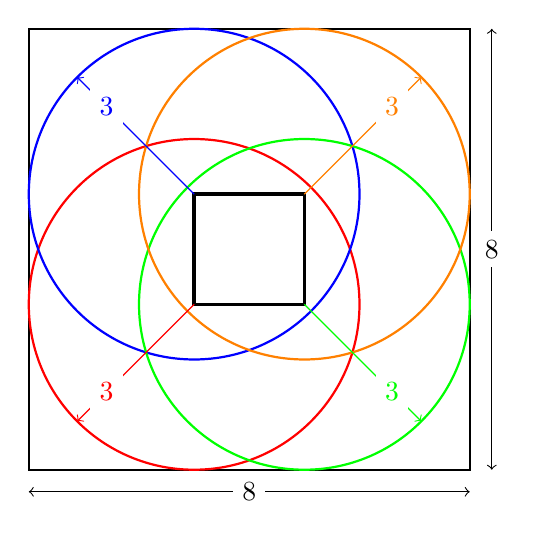
\begin{tikzpicture}[scale=.7]
\coordinate (c1) at (3,3);
\coordinate (c2) at (3,5);
\coordinate (c3) at (5,3);
\coordinate (c4) at (5,5);
\draw[very thick] (c1) -- (c3) -- (c4) -- (c2) -- cycle;
\draw[thick] (0,0) rectangle +(8,8);
\draw[color=red,thick] (c1) circle[radius=3];
\draw[color=blue,thick] (c2) circle[radius=3];
\draw[color=green,thick] (c3) circle[radius=3];
\draw[color=orange,thick] (c4) circle[radius=3];
\vertexcolor{c1}{red};
\vertexcolor{c2}{blue};
\vertexcolor{c3}{green};
\vertexcolor{c4}{orange};
\draw[<->] (0,-.4) -- node[fill=white] {$8$} (8,-.4);
\draw[<->] (8.4,0) -- node[fill=white] {$8$} (8.4,8);
\draw[->,red] (3,3) -- node[near end,fill=white] {$3$} +(-135:3);
\draw[->,blue] (3,5) -- node[near end,fill=white] {$3$} +(135:3);
\draw[->,green] (5,3) -- node[near end,fill=white] {$3$} +(-45:3);
\draw[->,orange] (5,5) -- node[near end,fill=white] {$3$} +(45:3);
\end{tikzpicture}
\end{center}
\caption{גבולות למטבעות שאינם חותכות את הריבוע}\label{f.coins1}
\end{figure}

\ans{2} התוחלת שלילית:
\[
E(\textrm{הטלה לכל הטלה})=5\cdot\frac{1}{16}\,+\,(-1)\cdot\frac{15}{16}=-\frac{10}{16}=-0.625\,.
\]

\ans{3}
איור%
~\ref{f.coins2}
מראה ארבעה מעגלים חסומים על ידי פינות הריבוע. הצלע של הריבוע הפנימית הוא 
$a-2r$
ולכן:
\[
P(\textrm{המעגל בתוך נוחת המטבע})=\frac{(a-2r)^2}{a^2}\,.
\]
\begin{figure}[tb]
\begin{center}
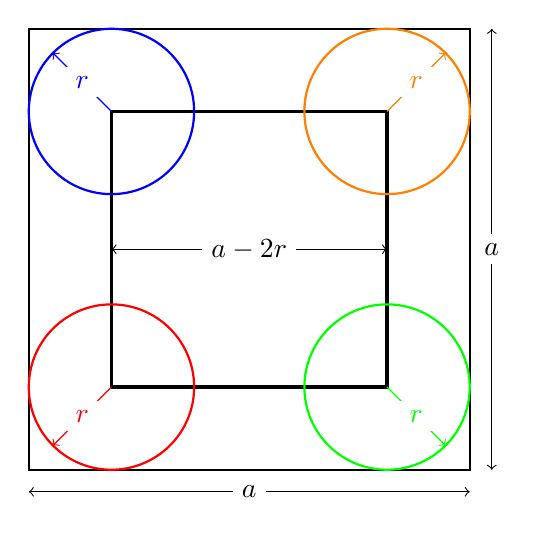
\begin{tikzpicture}[scale=.7]
\coordinate (c1) at (1.5,1.5);
\coordinate (c2) at (1.5,6.5);
\coordinate (c3) at (6.5,1.5);
\coordinate (c4) at (6.5,6.5);
\draw[very thick] (c1) -- (c3) -- (c4) -- (c2) -- cycle;
\draw[thick] (0,0) rectangle +(8,8);
\draw[color=red,thick] (c1) circle[radius=1.5];
\draw[color=blue,thick] (c2) circle[radius=1.5];
\draw[color=green,thick] (c3) circle[radius=1.5];
\draw[color=orange,thick] (c4) circle[radius=1.5];
\vertexcolor{c1}{red};
\vertexcolor{c2}{blue};
\vertexcolor{c3}{green};
\vertexcolor{c4}{orange};
\draw[<->] (0,-.4) -- node[fill=white] {$a$} (8,-.4);
\draw[<->] (8.4,0) -- node[fill=white] {$a$} (8.4,8);
\draw[->,red] (1.5,1.5) -- node[fill=white] {$r$} +(-135:1.5);
\draw[->,blue] (1.5,6.5) -- node[fill=white] {$r$} +(135:1.5);
\draw[->,green] (6.5,1.5) -- node[fill=white] {$r$} +(-45:1.5);
\draw[->,orange] (6.5,6.5) -- node[fill=white] {$r$} +(45:1.5);
\draw[<->] (1.5,4) -- node[fill=white] {$a-2r$} (6.5,4);
\end{tikzpicture}
\end{center}
\caption{מטבעות בריבוע גדול}\label{f.coins2}
\end{figure}

\textbf{סימולציה}
\selectlanguage{english}
\begin{verbatim}
For side = 8, radius = 1:
Probability of landing within the square = 0.5625
Proportion landing within the square     = 0.5704
For side = 8, radius = 2:
Probability of landing within the square = 0.2500
Proportion landing within the square     = 0.2481
For side = 8, radius = 3:
Probability of landing within the square = 0.0625
Proportion landing within the square     = 0.0639
For side = 8, radius = 4:
Probability of landing within the square = 0.0000
Proportion landing within the square     = 0.0000
\end{verbatim}
\selectlanguage{hebrew}

%%%%%%%%%%%%%%%%%%%%%%%%%%%%%%%%%%%%%%%%%%%%%%%%%%%%%%%%%%%%%

\begin{prob}{הטלת מזל}{S}{Chuck-a-luck}
בחר מספר 
$n$
בין 
$1$
ל-%
$6$.
הטל שלוש קוביות. אם לא מופיע
$n$
על אף קוביה אתה מפסיד
$1$;
אם 
$n$
מופיע על קוביה אחת אתה מרוויח
$1$;
אם 
$n$
מופיע על שתי קוביות אתה מרוויח
$2$;
אם 
$n$
מופיע על כל שלושת הקוביות אתה מרוויח 
$3$.
מה התוחלת של הרווח?
\end{prob}

\solution{}

תהי 
$P(k)$
ההסתברות ש-%
$n$
מופיע על 
$k$
קוביות. אזי:
\[
E(\textrm{הטלה לכל רווח})=-1 P(0) + 1 P(1) + 2 P(2) + 3 P(3)\,.
\]
ההטלות של שלושת הקוביה הן בלתי-תלויות ולכן כל ההסתברויות ניתנות על ידי ההתפלגות הבינומית עם 
$p=1/6$,
ההסתברות ש-%
$n$
מופיע על קוביה:
\begin{eqnarray*}
E(\textrm{הטלה לכל רווח}) &=& 
-1\dischoose{3}{0}\left(\frac{1}{6}\right)^0\left(\frac{5}{6}\right)^3
+1\dischoose{3}{1}\left(\frac{1}{6}\right)^1\left(\frac{5}{6}\right)^2+\\
&&2{3\choose 2}\left(\frac{1}{6}\right)^2\left(\frac{5}{6}\right)^1+
3\dischoose{3}{3}\left(\frac{1}{6}\right)^3\left(\frac{5}{6}\right)^0\\
&=& \frac{1}{216}(-125+75+30+3)\\
&=&-\frac{17}{216}\approx -0.0787\,.
\end{eqnarray*}

\textbf{סימולציה}
\selectlanguage{english}
\begin{verbatim}
Expectation of winnings = -0.0787
Average winnings        = -0.0724
\end{verbatim}
\selectlanguage{hebrew}

%%%%%%%%%%%%%%%%%%%%%%%%%%%%%%%%%%%%%%%%%%%%%%%%%%%%%%%%%%%%%

\begin{prob}{לרפא את המהמר הכפייתי}{S}{Curing the compulsive gambler}
רולט
\L{roulette}
הוא משחק מזל שמשחקים עם גלגל בעל 
$38$
כיסים ממוספרים:
$18$
אדומים,
$18$
שחורים ו-%
$2$
ירוקים.%
\footnote{ברולט אמריקאי נמצאים שני כיסים ירוקים וברולט אירופאי נמצא כיס ירוק אחד.}
מסובבים את הגלגל וכדור נוחת באחד הכיסים. הקזינו מנצח אם הכדור נוחת בכיס ירוק; אחרת, את מרוויחה 
$36$
עבור הימור של
$1$
על מספר הכיס (אדום או שחור) בו נוחת הכדור. את משחקת 
$36$
סבבים של רולט ומהממרת 
$1$
בכל סבב.

\que{1}
מה התוחלת  של הרווח?

\que{2}
חברך מציע להמר 
$20$
שאחרי 
$36$
סבבים את 
\textbf{תפסידי}
כסף. מה התוחלת של הרווח בהתחשב ברווח או הפסד של המשחק וגם של ההימור על חברך?
\end{prob}

\solution{}

\ans{1}
ההסתברות של ניצחון בסבב אחד היא
$1/38$
ולכן:
\begin{eqnarray*}
E(\textrm{אחד בסבב רווח})&=&35\cdot \frac{1}{38} + (-1)\cdot\frac{37}{38} = -\frac{2}{38} \approx -0.0526\\
E(\textrm{סבבים}\;36\textrm{ב- רווח })&=&36\cdot -0.05266=-1.8947\,.
\end{eqnarray*}
(הרווח נטו הוא 
$35$
כי ה-%
$36$
שאת מקבלת כולל החזרת ה-%
$1$
של ההימור.)

\ans{2}
נבדוק את ארבעת התוצאות של 
$36$
של משחק הרולט:
\begin{itemize}
\item
אם את מפסידה בכל הסבבים ההפסד הוא 
$36$.
\item
אם את מנצחת בסבב אחד ומפסידה ב-%
$36$
סבבים אין רווח ואין הפסד.
\item
אם את מנצחת בשני סבבים את מרוויחה 
$70$
ומפסידה 
$34$
בשאר הסבבים כך שהרווח נטו הוא
$36$.
\item 
אם את מנצחת ב-%
$k$
עבור
$2<k\leq 36$,
הרווח נטו הוא
$35k - (36-k)>0$.
\end{itemize}
לכן את הפסידה כסף רק אם את מפסידה את כל הסבבים:
\[
P(\textrm{סבבים} \;36 \textrm{ב- מפסידה})=\left(\frac{37}{38}\right)^{36}\approx 0.3829\,.
\]
ההסתברות לא להפסיד בכל הסבבים היא 
$1-0.3829=0.6171$.
לכן:
\[
\overbrace{-1.8947}^{\textrm{\small הסבבים כל של E}}+\;\;
\overbrace{-20\cdot 0.3829}^{\textrm{\small בהימור מפסידה}} \;+\; \overbrace{20\cdot 0.6171}^{\textrm{\small בהימור מנצחת}} \approx 2.7904\,.
\]
ברור שכדאי להסכים להימור המוצע!

\textbf{סימולציה}
\selectlanguage{english}
\begin{verbatim}
Expectation of winning a round = -0.0526
Average winnings for a round   = -0.0593
\end{verbatim}
\selectlanguage{hebrew}
בסימוליה היתה שונות גדולה שהוקטנה כל ידי הרצת מיליון ניסויים.

%%%%%%%%%%%%%%%%%%%%%%%%%%%%%%%%%%%%%%%%%%%%%%%%%%%%%%%%%%%%%

\begin{prob}{קלפים מושלמים בברידג'}{}{Perfect bridge hand}
בחר באקראי 
$13$
קלפים בחבילה של 
$52$
קלפים. מה ההסתברות שכולם מאותה סדרה?
\end{prob}

\solution{1}

בכל חבילה יש 
$13$
קלפים מכל סדרה כך שיש 
$\dischoose{52}{13}$
דרכים לבחור 
$13$
מסדרה אחת, למשל, לבבות. יש רק דרך אחת לבחירת 
$13$
לבבות כך ש:
\[
P(\textrm{לבבות}\;13\;\textrm{בחירת})=\frac{1}{\dischoose{52}{13}}=\frac{13! 39!}{52!}=\approx 1.5747\times 10^{-12}\,.
\]
בחבילה ארבע סדרות ולכן:
\[
P(\textrm{סדרה מאותה קלפים}\;13\;\textrm{בחירת })=4\cdot \frac{13! 39!}{52!}\approx 6.2991\times 10^{-12}\,.
\]

\solution{2}

יש 
$52$
דרכים לבחור את הקלף הראשון. אח"כ יש 
$12$
דרכים לבחור את הקלף השני מאותה סדרה מתוך 
$51$
הקלפים שנשארו,
$11$
דרכים לבחור את הקלף השלישי, וכו'. מכאן:
\[
P(\textrm{סדרה מאותה קלפים}\;13\;\textrm{בחירת})=\frac{52}{52}\cdot \frac{12}{51}\cdot \frac{11}{50} \cdots  \frac{1}{40}= \frac{12!}{51!/39!}\approx 6.2991\times 10^{-12}\,.
\]
אין טעם להריץ סימולציה כי כמעט בוודאות התוצאה תהיה אפס.

%%%%%%%%%%%%%%%%%%%%%%%%%%%%%%%%%%%%%%%%%%%%%%%%%%%%%%%%%%%%%

\begin{prob}{משחק קוביות}{D,S}{Craps}
משחק ה-%
\L{craps}
הוא משחק עם זוג קוביות. בהטלה הראשונה אתה מנצח אם סכום המספרים הוא
$7$
או
$11$,
ואתה מפסיד אם הסכום הוא
$2$, $3$
או
$12$.
אם הסכום בהטלה הראשונה הוא
$n=4,5,6,8,9,10$ 
(נקרא "נקודה" 
\L{point}),
המשך להטיל את הקוביות עד שמופיעה הנקודה 
$n$
(ניצחון) או 
$7$
(הפסד).

\que{1} 
מה ההסתברות של האירועים בהטלה הראשונה: ניצחון, הפסד, לא ניצחון ולא הפסד?

\que{2} 
מה ההסתברות לניצחון?
\end{prob}

\solution{1}

\ans{1}
להסתברות של המספרים המופיעים כאשר מטילים קוביה התפלגות אחידה השווה ל-%
$1/6$.
ההטלות של שתי קוביות בלתי תלויות ולכן ההסתברות של כל תוצאה היא 
$1/36$.
מספר הדרכים לקבל כל אחד מהאירועים (הסכום של זוג קוביות)
$2,\ldots,12$
הוא:
\[
\begin{array}{rrrrrrrrrrr|l}
2 & 3 & 4 & 5 & 6 & 7 & 8 & 9 & 10 & 11 & 12&\textrm{סכום}\\\hline
 1 & 2 & 3 & 4 & 5 & 6 & 5 & 4 & 3 & 2 & 1&\textrm{זוגות}
\end{array}
\]
בהטלה הראשונה יש 
$8$
דרכים לקבל
$7$
או
$11$
וההסתברות היא
$8/36$
לנצח. יש
$4$
דרכים לקבל
$2,3,12$
וההסתברות היא 
$4/36$.
ההסתברות לא לנצח ולא להפסיד היא בהטלה הראשונה היא:
\[
1 - \frac{8}{36} - \frac{4}{36} = \frac{24}{36}\,.
\]

\ans{2}
נעיין בשני מקרים תוך התייחסות לטבלה לעיל:
\begin{itemize}
\item 
הנקודה היא
$4$.
ההסתברות לנצח בהטלה השנייה ($4$) היא
$3/36$
וההסתברות להפסיד ($7$) היא
$6/36$.
ההסתברות לא לנצח ולא להפסיד היא
$1-(3/36)-(6/36)=27/36$.

\item
הנקודה היא $8$. ההסתברות לנצח בהטלה השנייה ($8$) היא
$5/36$
וההסתברות להפסיד ($7$) היא
$6/36$.
ההסתברות לא לנצח ולא להפסיד היא
$1-(5/36)-(6/36)=25/36$.
\end{itemize}
אנו רואים שחייבים לחשב את ההסתברות לנצח בנפרד עבור כל אחת מהנקודות 
$4,5,6,8,9,10$.
נפתח נוסחה כללית להסתברות.

לאחר שהתקבל
\textbf{הנקודה}
$n$
בהטלה הראשונה, תהי 
$P_n$
ההסתברות ההסתברות לנצחון על ידי הטלת הנקודה 
$n$
בהטלה כשלהי, ותהי
$Q_n$
ההסתברות לא לנצח ולא להפסיד בהטלה כלשהי.
תהי
$W_n$ 
ההסתברות לנצחון על ידי הטלת הנקודה 
$n$
\textbf{בהטלה לאחר ההטלה הראשונה}.
ניתן לחשב את
$W_n$ 
על ידי חיבור:
\begin{itemize}
\item 
ההסתברות להופעת הנקודה בהטלה השנייה. 
\item 
ההסתברות לא לנצח ולא להפסיד בהטלה השנייה כפול ההסתברות להופעת הנקודה בהטלה השלישית.
\item 
ההסתברות לא לנצח ולא להפסיד בהטלה השנייה והשלישית כפול ההסתברות להופעת הנקודה בהטלה הרביעית,
\end{itemize}
וכך הלאה.
\begin{eqnarray*}
W_n&=&P_n + Q_n P_n + Q_n^2 P_n+ Q_n^3 P_n  + \cdots\\
&=&P_n\left(1+Q_n^1 + Q_n^2+ Q_n^3  + \cdots\right)\\
&=&P_n\left(\frac{1}{1-Q_n}\right)\,.
\end{eqnarray*}
אתה מפסיד אם בהטלה כלשהי לאחר הראשונה מופיע 
$7$
עם הסתברות
$6/36$
ולכן:
\begin{eqnarray*}
Q_n &=& 1-P_n-(6/36)\\
W_n&=&\frac{P_n}{P_n+(6/36)}\,.
\end{eqnarray*}
$W_n$
עבור ששת הנקודות היא:
\[
\renewcommand{\arraystretch}{2}
\begin{array}{lcccccc}
n   & 4 & 5 & 6 & 8 & 9 & 10 \\\hline
P_n & \disfrac{3}{36} & \disfrac{4}{36} & \disfrac{5}{36} & \disfrac{5}{36} & \disfrac{4}{36} & \disfrac{3}{36} \\
%1-Q_n & \disfrac{9}{36} & \disfrac{10}{36} & \disfrac{11}{36} & \disfrac{11}{36} & \disfrac{10}{36} & \disfrac{9}{36} \\
W_n & \disfrac{3}{9} & \disfrac{4}{10} & \disfrac{5}{11} & \disfrac{5}{11} & \disfrac{4}{10} & \disfrac{3}{9}
\end{array}
\]
ניתן לחשב את
$W$, 
ההסתברות לנצח, על ידי חיבור ההסתברות לנצח בהטלה הראשונה לסכום ההסתברויות עבור ששת הנצחונות בהטלת נקודה כפול ההסתברות להופעת 
\textbf{אותה נקודה}
בהטלה הראשונה:
\begin{equation}\label{eq.9-a}
W=\frac{8}{36}+\sum_{n\in\{4,5,6,8,9,10\}} P_nW_n \approx 0.4929\,.
\end{equation}
שסיכוי שהקזינו ינצח במשחק אחד של 
\L{craps}
הוא רק
$0.5-0.4949\approx 0.5\%$
אבל חוק המספרי הגדולים מבטיח שבסופו של דבר הם ינצחו ואתה תפסיד!

\solution{2}

\ans{2}
נעיין בסדרות ההטלות שלהן כאשר בכולן הנקודה היא
$4$. 
\[
\begin{array}{rrrrrrrrrrr}
4 & 8 & 9 & 9 & 9 & 8 & 8 & 8 & 9 & 8 & 4\\
4 & 8 & 9 & 9 & 9 & 8 & 8 & 8 & 9 & 8 & 7\\
4 & 9 & 9 & 9 & 8 & 8 & 4
\end{array}
\]
המשחק מסתיים רק אם מטילים 
$4$
(ניצחון) או מטילים
$7$
(הפסד), כך שהופעות של 
$8$
או
$9$
לא משפיעות על התוצאה. מכאן שהסתברות לנצח היא ההסתברות המותנית שמופיע
$4$
אם נתון שהופיע
$4$
או
$7$. 
יהי 
$f$
האירוע ש-%
$4$
מופיע ויהי
$s$
האירוע ש-%
$7$
מופיע. אזי:
\[
P(f|f\cup s) = \disfrac{P(f)\cap P(f\cup s)}{P(f\cup s)}=\disfrac{P(f)}{P(f\cup s)}=\disfrac{3/36}{(3+6)/36}=\disfrac{3}{9}\,,
\]
בדיוק התוצאה 
$W_4$
שמופיעה בטבלה לעיל. כעת ניתן להשתמש במשוואה%
~\ref{eq.9-a}
כדי לחשב את
$W$.

השתמשנו בהסתברות בצורה סמויה בפתרון הראשון כי 
$W_n$
היא ההסתברות המותנית שבהטלה הראשונה מופיעה הנקודה
$n$.

\textbf{סימולציה}
\selectlanguage{english}
\begin{verbatim}
Probability of winning = 0.4929
Proportion of wins     = 0.4948
\end{verbatim}
\selectlanguage{hebrew}

%%%%%%%%%%%%%%%%%%%%%%%%%%%%%%%%%%%%%%%%%%%%%%%%%%%%%%%%%%%%%

\refstepcounter{problem}  % 10. An experiment in personal taste
